%% Referee Version
\documentclass[referee,sn-basic]{sn-jnl} % referee option is meant for double line spacing

%% Final Version
%%\documentclass[sn-mathphys-num]{sn-jnl} % Math and Physical Sciences Numbered Reference Style 

%%%% Standard Packages
\usepackage{graphicx}%
\usepackage{multirow}%
\usepackage{amsmath,amssymb,amsfonts}%
\usepackage{amsthm}%
\usepackage{mathrsfs}%
\usepackage[title]{appendix}%
\usepackage{xcolor}%
\usepackage{textcomp}%
\usepackage{manyfoot}%
\usepackage{booktabs}%
\usepackage{algorithm}%
\usepackage{algorithmicx}%
\usepackage{algpseudocode}%
\usepackage{listings}%
\usepackage{physics}% added to use braket notation

%%% To be removed once finished
\newcommand{\todo}[1]{\textcolor{green}{[TODO: #1]}}

\begin{document}

\title[Quantum Circuits Noise Simulation with Reinforcement Learning]{Quantum Circuits Noise Simulation with Reinforcement Learning}

\author*[1,2,4]{\fnm{Simone} \sur{Bordoni}}\email{simone.bordoni@uniroma1.it}

\author[2,4]{\fnm{Andrea} \sur{Papaluca}}\email{andrea.papaluca@anu.edu.au}
\equalcont{These authors contributed equally to this work.}

\author[1,2]{\fnm{Piergiorgio} \sur{Buttarini}}\email{add@email.com}
\equalcont{These authors contributed equally to this work.}

\author[2,5]{\fnm{Alejandro} \sur{Sopena}}\email{add@email.com}
\equalcont{These authors contributed equally to this work.}

\author[2,6]{\fnm{Stefano} \sur{Carrazza}}\email{add@email.com}

\author[1,4]{\fnm{Stefano} \sur{Giagu}}\email{stefano.giagu@uniroma1.it.com}

\affil[1]{\orgdiv{Dep. of Physics}, \orgname{La Sapienza University of Rome}, \orgaddress{\street{Piazzale Aldo Moro 2}, \city{Rome}, \postcode{00185}, \state{Italy}}}

\affil[2]{\orgdiv{Quantum Research Center}, \orgname{Technology Innovation Institute}, \orgaddress{\street{Masdar City}, \city{Abu Dhabi}, \postcode{9639}, \state{United Arab Emirates}}}

\affil[3]{\orgdiv{School of Computing}, \orgname{The Australian National University}, \orgaddress{\street{108 North Rd}, \city{Canberra}, \postcode{2601}, \state{Australia}}}

\affil[4]{\orgdiv{Sez. di Roma}, \orgname{INFN}, \orgaddress{\street{Piazzale Aldo Moro 2}, \city{Rome}, \postcode{00185}, \state{Italy}}}

\affil[5]{\orgdiv{Instituto de Fisica Teorica, UAM/CSIC}, \orgname{Universidad Autonoma de Madrid}, \orgaddress{\street{C. Nicolás Cabrera 13-15}, \city{Madrid}, \postcode{28049}, \state{Spain}}}

\affil[6]{\orgdiv{TIF Lab}, \orgname{Università degli Studi di Milano}, \orgaddress{\street{Via Celoria 16}, \city{Milan}, \postcode{20133}, \state{Italy}}}


%%==================================%%
%% Sample for unstructured abstract %%
%%==================================%%

\abstract{Quantum computing in the NISQ era requires powerful tools to reduce the gap between simulations and quantum hardware execution. In this work, we present a machine learning approach to characterize a noise model and reproduce it during simulations. The proposed algorithm is based on reinforcement learning and is meant to be more flexible, in reproducing different models of noise, than standard techniques like randomized benchmarking or heuristic noise models. We have tested the proposed model both with simulations and on real superconducting qubits. We also include two use-case examples. The first is a simulation of a noisy circuit to implement a quantum Fourier transform, the second is an application to quantum machine learning.}

\keywords{keyword1, Keyword2, Keyword3, Keyword4}

%%\pacs[JEL Classification]{D8, H51}

%%\pacs[MSC Classification]{35A01, 65L10, 65L12, 65L20, 65L70}

\maketitle
\section{Introduction}
One important unsolved technological questions is whether Noise Intermediate Scale Quantum (NISQ)~\cite{Preskill_2018} computers will be useful for practical applications. In fact, quantum computers are expected to offer speedups over classical computers in certain computational tasks~\cite{Shor_1997, grover1996fast, Zhong_2020}. However, NISQ devices are limited in usability and reliability mainly because of errors due to: gate infidelities, unwanted interactions with the environment, thermal relaxation, measurement errors and cross-talk~\cite{PhysRevLett.121.090502, doi:10.1146/annurev-conmatphys-031119-050605, PRXQuantum.3.020301, PhysRevB.104.045420, 9355264}. Hence, it is widely regarded that near-term quantum advantage will only be achieved through advanced error mitigation techniques~\cite{PRXQuantum.2.040326, PhysRevA.105.062404, 10.1145/3352460.3358265, Sopena_2021, PRXQuantum.2.040330} or only with the future generations of fault-tolerant quantum devices~\cite{article_knill, PhysRevX.8.021054, PhysRevA.86.032324, Varsamopoulos_2017, bordoni2023}.
Even if no advantage has been proven on NISQ devices, many algorithms have been developed and deployed on this hardware. In particular machine learning inspired models has shown encouraging results in the last years~\cite{Biamonte_2017, 8939749, Cerezo_2021, egger2023study, particles6010016, Robbiati:2853183, robbiati2022quantum, cruzmartinez2023multivariable}.
In order to study these kind of algorithms it is important to be able to emulate their behavior when executed on imperfect quantum chips. In this work we want to develop a model able to learn a hardware specific noise to be used for predictions during circuit simulations. This objective is further motivated by the fact that very few techniques of noise modeling or noise prediction are available to this date~\cite{zlokapa2020deep, inproceedings_caracterization, PhysRevA.104.062432, Harper_2020}.
In our approach we train an agent with Reinforcement Learning (RL)~\cite{sutton2018reinforcement, kaelbling1996reinforcement, wiering2012reinforcement}, in order to add noise channels to reproduce the noise pattern of a specific quantum chip. In this way we reduce as much as possible the heuristic assumption on the noise model, thus increasing the adaptability and generalization properties of the algorithm.\\

\noindent
This article is structured as follows:\\
In Section~\ref{sec_background} we introduce the basic concepts necessary to understand the proposed algorithm, reinforcement learning and the noise in quantum circuits. \\
In Section~\ref{sec_methodology} we describe in detail the reinforcement learning algorithm, with particular regard to its training and its use for noise prediction. \\
Section~\ref{sec_results} reports the results obtained with the proposed algorithm both on simulations and on real quantum devices, the performance is also compared with other noise predictors. \\
In Section~\ref{sec_applications} we show examples use-cases of the algorithm for quantum machine learning and quantum Fourier transform applications.

\section{Background}\label{sec_background}
In this section we want to review the main topics necessary to understand the proposed noise simulation algorithm.
In particular we will give a brief introduction to reinforcement learning and the noise in quantum circuits.

\subsection{Reinforcement learning}\label{sec_rl}
Reinforcement learning is a powerful paradigm in Machine Learning (ML) that deals with the training of an agent to make optimal decisions in a dynamic environment. From a mathematical perspective a RL algorithm is described as a Markov Decision Process (MDP)~\cite{PUTERMAN1990331}. In a MDP the future state depends solely on the current state and action, regardless of the history of previous states and actions. MDPs rely on the fundamental concepts of policy, reward functions and discount factors. The policy determines the behavior of the agent mapping the states of the environment to actions. The reward function assigns a numeric value to state-action pairs, indicating the immediate desirability or cost associated with them. The discount factor balances the importance of immediate rewards against future rewards, allowing for consideration of long-term consequences. Solving MDPs involves finding an optimal policy that maximizes the expected cumulative reward.
In a RL model the policy is implemented by an artificial Neural Network~\cite{Zou2009} (NN). In order to train the NN different episodes of agent-environment interaction are executed. At the end of each episode (or batch of episodes) the cumulative reward is computed and is used to update the weights of the NN using the backpropagation algorithm~\cite{Rojas1996}.\\
In recent years many different optimization methods have been developed to improve RL convergence and stability during training~\cite{ozalp2020}. In our work we have obtained the best results using the Proximal Policy Optimization (PPO)~\cite{schulman2017proximal}. This optimization method provides an increased stability by constraining the policy update to a proximity region. Moreover PPO is able to handle a continuous action space, necessary to accurately model quantum noise. One drawback is its sensitivity to hyperparameters, poorly chosen values can impact convergence and overall performance. In order to define and train the algorithm we have used the library \textit{Stable\_Baselines3}~\cite{JMLR:v22:20-1364}. This library is built on top of \textit{OpenAI Gym}~\cite{article_gym} which provides a wide range of customizable environments for reinforcement learning tasks. Gradient optimization has been performed with \textit{pytorch}~\cite{NEURIPS2019_9015}.

\subsection{Noise in quantum circuits}
Quantum noise is a crucial challenge faced in quantum circuits, which can significantly impact the expected results of computations on NISQ hardware. Qubits are susceptible to various sources of noise, such as environment interaction, spontaneous emission or calibration errors. Errors accumulate during the execution of a quantum circuit making the final result less accurate or even completely erroneous. Many mathematical tools have been developed in order to describe quantum noise~\cite{PhysRev.121.920, nielsen_chuang_2010, 10.1117/12.2017396}. In this work we will model quantum noise using error channels, which are represented as superoperators acting on state density matrices. The following list provides a concise overview of the error channels utilized in this study:
\begin{description}
    \item[Depolarizing:] this channel acts uniformly on all possible quantum states. Depolarization refers to the flattening or averaging of the quantum state, making it less distinguishable from other possible states, leading to a loss of coherence and entanglement. Depolarization is typically quantified by a parameter $\lambda$, which represents the probability of an error occurring in the transmission or processing of the state. The depolarizing channel act on a single qubit state $\rho$ as follows:
    \begin{equation*}
    Dep_\lambda(\rho)=(1-\lambda)\rho+\lambda\mathbb{I}.
    \end{equation*}
    
    \item[Amplitude Damping:] this channel models physical processes, occurring on the qubits, that involve energy dissipation or spontaneous emission. The amplitude damping channel describes a decay process where the state $\ket{0}$ is conserved while $\ket{1}$ decays to $\ket{0}$ with probability $\gamma$:
    \begin{equation*}
    Damp(\gamma)\ket{1}=(1-\gamma)\ket{1}+\gamma\ket{0}
    \end{equation*}
    This channel is similar to the thermal relaxation channel but does not take into account the phase decoherence. We decided to use the amplitude damping because, even if less general, it needs a single parameter instead of the three parameters necessary to describe the thermal relaxation. This makes the training of the RL agent easier and less prone to overfitting. Moreover, we have not noticed any significant performance reduction when applying this channel instead of the thermal relaxation during preliminary tests.
    
    \item[Coherent errors:] this kind of errors are unitary and can be represented with single qubit rotation gates ($R_x$, $R_y$, $R_z$). They can arise for several reasons like a wrong calibration, cross-talk, external fields, and residual qubit–qubit interactions~\cite{Cenedese_2023}. For example, when a rotation gate ($R(\theta)$) is applied, a coherent error can introduce an unwanted perturbation in the rotation angle ($R(\theta+\epsilon)$). Because of their different nature, coherent errors can have strong effects on quantum error correction codes~\cite{Greenbaum_2017, Venn_2023, Beale_2018}. On the other hand, as these errors do not destroy quantum information, once identified, they can be corrected~\cite{Cenedese_2023, Kern_2005, Bravyi_2018}.
\end{description}
\noindent
Different noise channels can be combined in order to create complex noise models~\cite{PhysRevA.104.062432, article_model_realistic}. The parameters of the channels can be inferred from calibration results or directly from quantum circuits execution like in this work.
In order to obtain a simple modeling of the noise, it is possible to use a technique called Randomized Benchmarking (RB)~\cite{Emerson_2005, heinrich2023randomized, 2019npj}.
With RB it is possible to estimate the magnitude of the average error in a set of quantum gates. This estimation can be performed in an efficient way, resources required scale polynomially with the number of qubits in the device. The general idea behind RB is that of applying sequences of randomly chosen quantum gates of varying length. Small errors are thus amplified with the sequence length, and gate quality measures can be extracted from the dependence of the output data on sequence length.
The noise model obtained in this way is unrealistic as all noise sources are projected on the depolarizing channel. However, this technique allows to compute a good average gate fidelity and can be used as a basic benchmark for other, more sophisticated, noise characterization techniques.

\section{Methodology}\label{sec_methodology}
In this section we will describe the proposed noise modeling algorithm. The main focus is given to the dataset generation and the training procedure. These steps are similar for both quantum circuit simulations and execution on real quantum hardware. For the simulation phase we have used \textit{Qibo}~\cite{Efthymiou_2021}, an open-source software for fast evaluation of quantum circuits.

\subsection{Dataset generation}\label{sec_dataset}
In order to train a RL algorithm it is necessary to generate train, test and evaluation datasets.
All these datasets are composed of ensembles of random quantum circuits with their relative Density Matrices (DM). DMs are used as ground truth labels during the training of the algorithm (Section~\ref{sec_training}). DMs are analytically computed in simulations.  When circuits are executed on hardware, they can be extracted using quantum state tomography~\cite{PhysRevLett.109.120403}, or more efficient techniques like classical shadow state reconstruction~\cite{PRXQuantum.2.010307, Eisert_2020, PRXQuantum.2.030348}.\\ 
For the training and test sets, circuits have been generated with a fixed number of moments. A moment is a collection of gates that can be executed in parallel. The total number of moments in a quantum circuit is called depth.  The evaluation datasets, used for performance benchmarking, are composed of circuits with different depths. For the datasets used for simulations it is possible to define a custom noise model, this will be described with accuracy in Section~\ref{sec_simulation}. All the datasets circuits have been generated by extracting random Clifford gates from among all the natives gates. We have used Clifford gates because of their good properties related to randomized benchmarking and shadow state estimation~\cite{2019npj, PhysRevA.77.012307, Eisert_2020, PRXQuantum.2.030348}.
The natives gates set is hardware specific and is composed of all gates that can be executed directly on hardware. For example, for this work, we have used the natives gates set of the Technology Innovation Institute (TII) quantum hardware, composed of $R_x$, $R_z$ and $CZ$ gates\footnote{TII quantum hardware uses $R_z$ and $GPI2$ as single qubit native gates. However, this last gate is equal to $R_x(\pi/2)$.}. It is important to notice that $R_x$ and $R_z$ are Clifford gates only when the rotation parameter is a multiple of $\pi/2$. We have also performed some preliminary tests with the IBM quantum hardware natives gates set~\cite{Santos_2016}, that uses the $CNOT$ gate as the two-qubits interaction native gate. Changing the natives gates is an easy procedure in the proposed algorithm and has not shown any significant performance change.\\

\noindent
In order to train the RL agent it is necessary to represent the quantum circuit as an array, that can be used as input of the policy neural network. We will call this array the quantum circuit representation (QCR). 
In the general case the shape of the QCR is:
\begin{equation*}
    [ \, qubits, \: depth, \:  encoding\_dim \, ].
\end{equation*}
Where $encoding\_dim$ depends on the number of primitive gates and the number of noise channels. 
The first entrance of QCR identifies the circuit qubit, while the second entrance identifies the circuit moment.
The $encoding\_dim$ is used to store the information of gates and noise channels acting on a specific qubit and circuit moment in the following way:
\begin{itemize}
    \item The first $n$ entrances are set to one in the presence of a single qubit gate, zero otherwise. In our work $n=2$, to encode the presence of an $R_x$ or $R_z$ gate.
    \item The entrance $n+1$ encodes the presence of a two qubit gate ($1$ if a $CZ$ is present, $0$ otherwise). For single qubit circuits this entrance is always set to zero.
    \item The $n+2$ entrance encodes the rotation angle of single qubit gates, its value is set to zero if no rotation gate is present. Rotation angles have been divided by $2\pi$ in order to set them in the interval $[0,1]$.
    \item The remaining entrances report the parameters of the noise channels in the following order: Depolarizing channel, Amplitude damping channel, $R_z$ coherent error and $R_x$ coherent error. If no noise channel is present the respective parameter value is set to zero. 
\end{itemize}
Figure~\ref{fig_qcr} reports an example of the QCR of a circuit with two qubits obtained with this procedure.
\begin{figure}
    \centering
    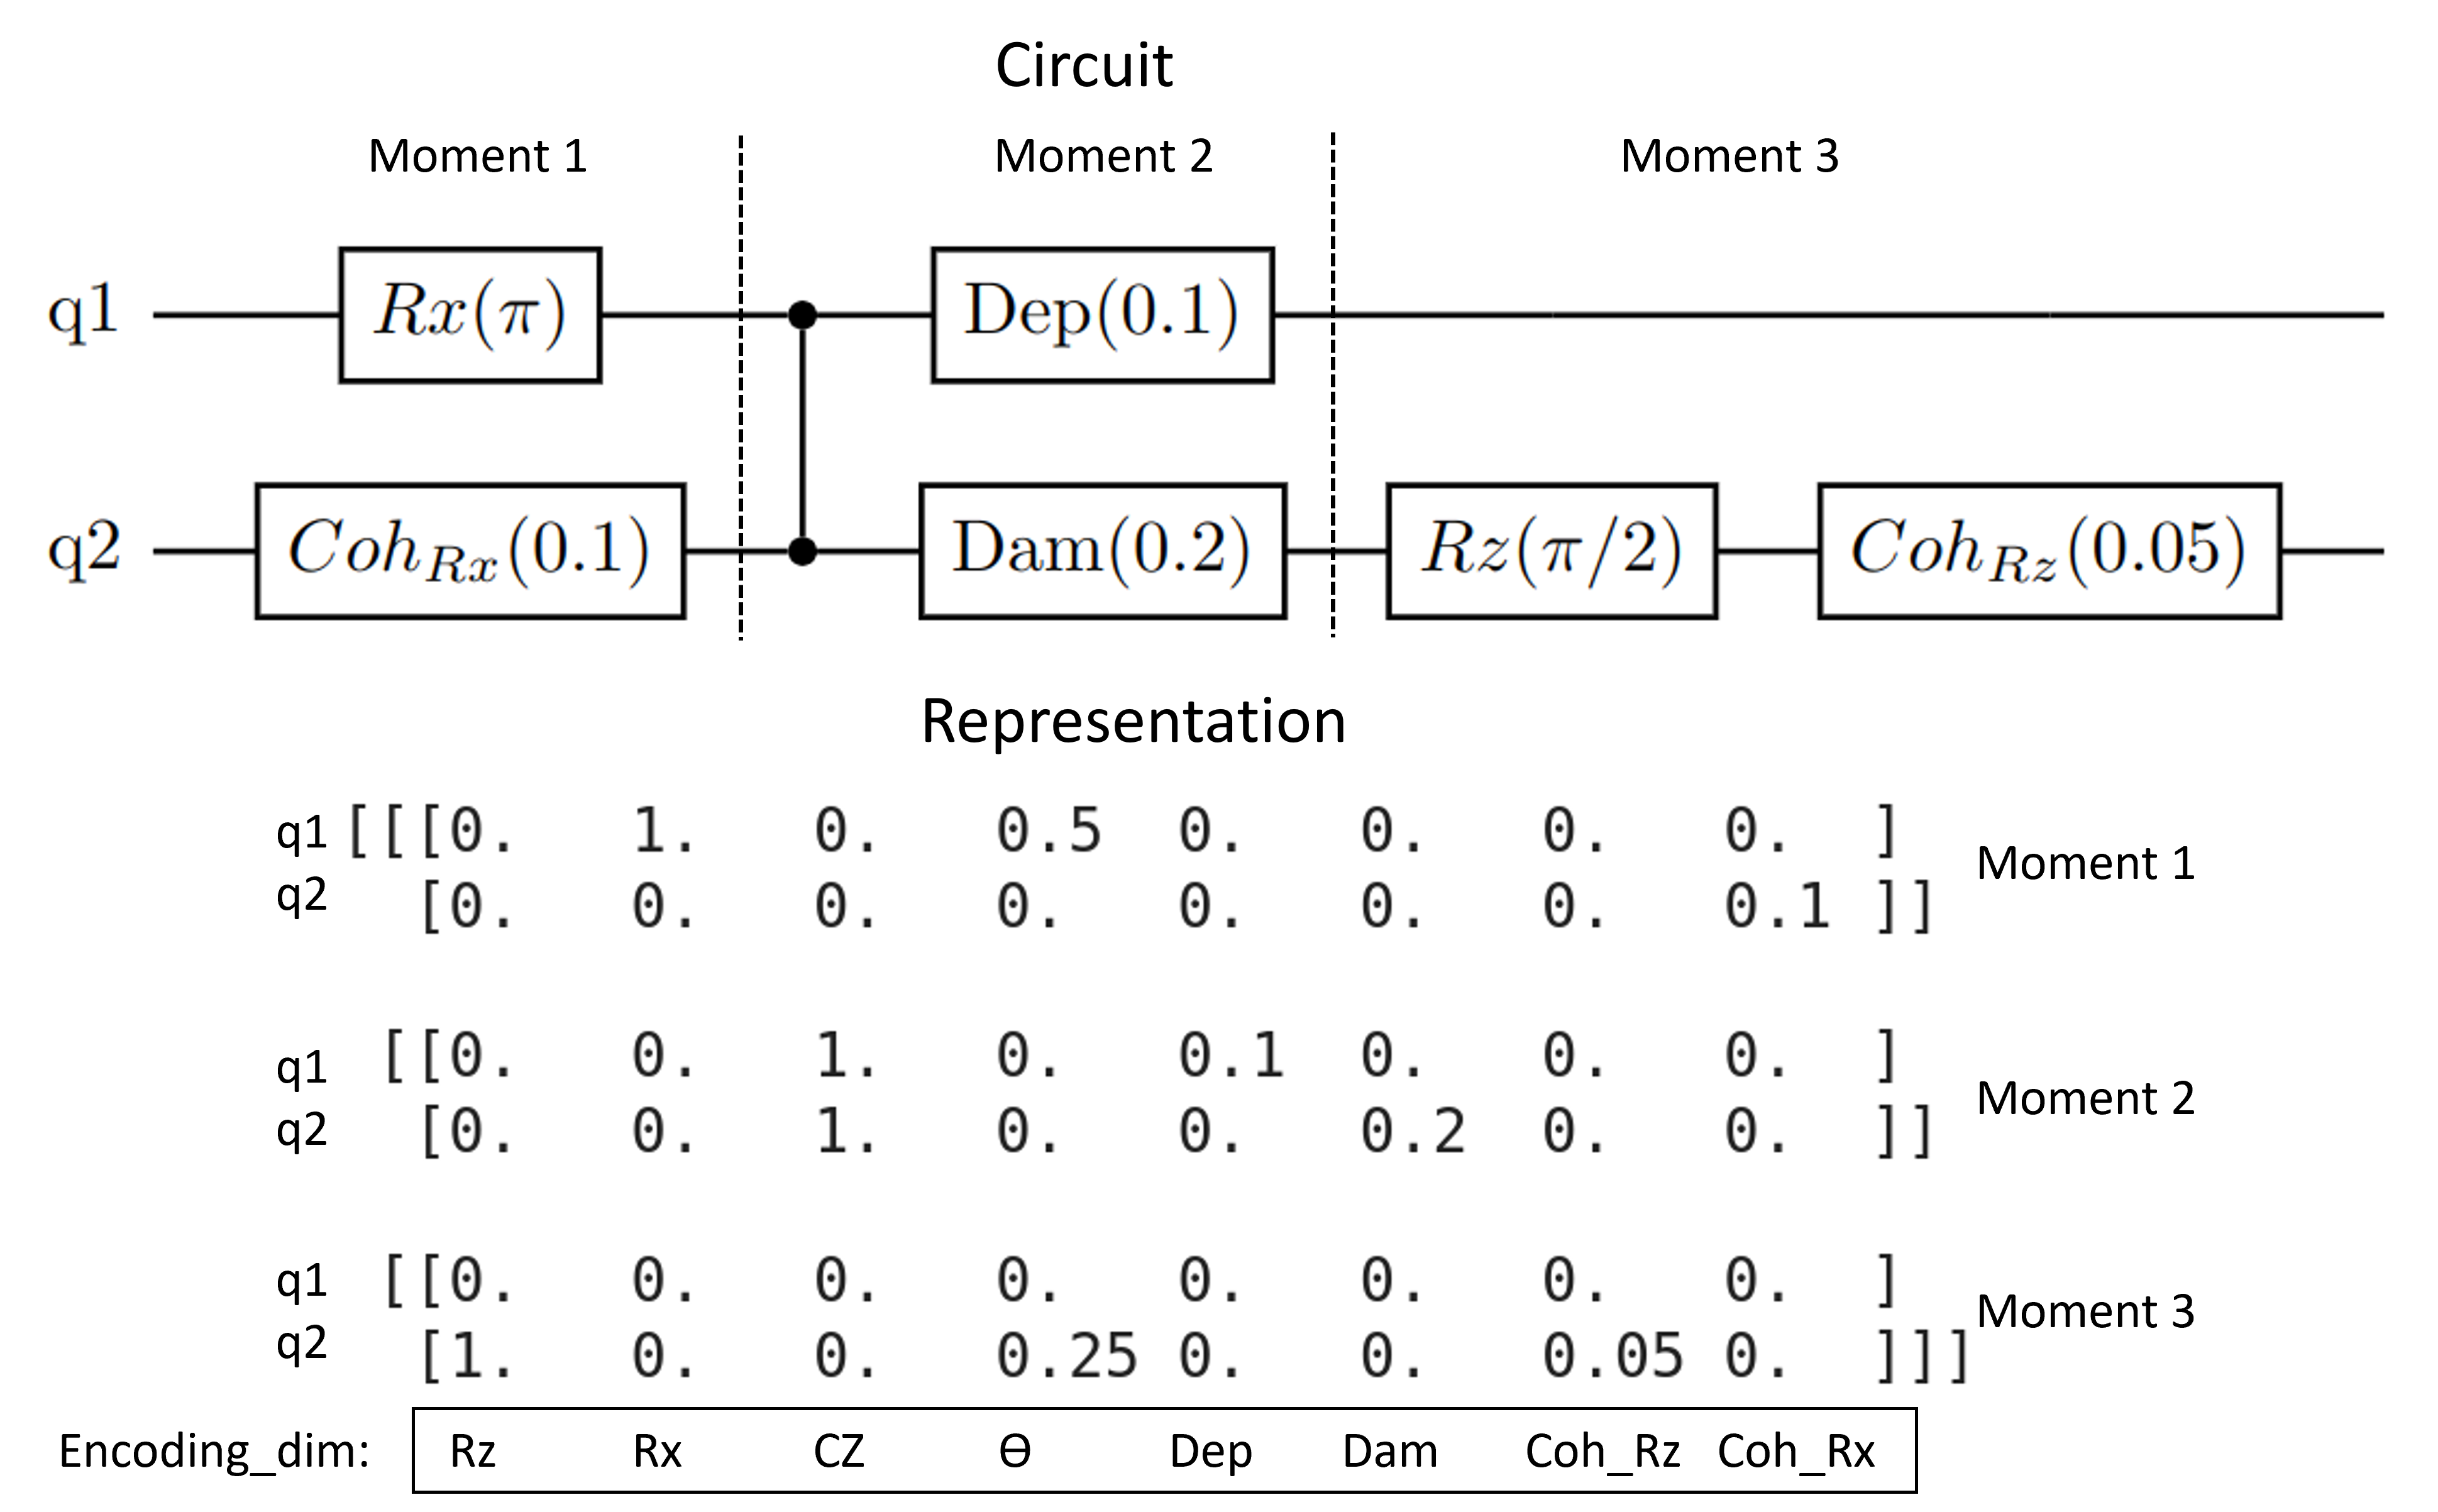
\includegraphics[width=0.49\textwidth]{circuit_representation.png}
    \caption{Example of the quantum circuit representation used in this work for a two qubit quantum circuit. }\label{fig_qcr}
\end{figure}

\subsection{Training procedure}\label{sec_training}

\begin{algorithm*}
\caption{Training procedure}\label{alg:train}
\begin{algorithmic}
\For{$episode$ in $n\_episodes$}
    \State{$circuit$ = random\_extraction($training\_set$)}
    \For{$moment$ in $circuit$}
        \State{$observation$ = $agent$.make\_observation($circuit$, $moment$)}
        \State{$action$ = $agent$.action($observation$)}
        \State{$circuit$.add\_noise($action$)}
    \EndFor
    \State{$generated\_dm$ = extract\_density\_matrix($circuit$)}
    \State{$reward$ = compute\_reward($generated\_dm$, $ground\_truth\_dm$)}
    \State{$agent$.update\_policy($reward$)}
\EndFor
\end{algorithmic}
\end{algorithm*}

The task of the RL agent is to learn and being able to reproduce a specific noise pattern. This is achieved with the following steps.\\
A non noisy, QCR is given to the agent at the beginning of each episode (random extraction from the training set). For every circuit moment the agent performs an observation of the circuit and makes an action that consists in putting any number of noise channels with a chosen parameter. At the end of an episode the DM of the circuit obtained with this process is computed (generated DM). The generated DM is compared with the real noisy circuit DM (Section~\ref{sec_dataset}), their fidelity is used to compute the final reward and update the weights of the policy NN (Section~\ref{sec_rl}).
After many episodes the agent should learn, in principle, where to put noise channels in a non-noisy circuit in order to reconstruct the DM of the real noisy circuit. 
A summary of this training procedure is reported in Algorithm~\ref{alg:train}. Once trained, the proposed algorithm should be able to generalize to previously unseen circuits to be used to perform realistic noisy simulations.\\

\noindent
Below is reported a description of the main elements of the RL algorithm employed in the training process.
\begin{description}
    \item[Observation:] performing an observation returns the feature vector that is given to the policy NN to decide the next. The observation shape is: 
    $$[\,qubits,\: kernel\_size,\: encoding\_dim\,].$$
    The first and the latter parameter where already described in Section~\ref{sec_dataset}. The $kernel\_size$ parameter has been introduced to make the agent adapt to circuits of different length, and has a similar role to the kernels used in convolutional neural networks~\cite{GU2018354}. The $kernel\_size$ defines a "window" that has the role of limiting how many moments of the circuit the agent can see for each observation. For example, if $kernel\_size=3$ at each step the agent will observe only the current moment, the previous and the next one. The center of the window start from the first moment and slides of a position at each step until the end of the circuit is reached. This implementation is motivated by the heuristic assumption that the noise on a gate is influenced more by the gates that are executed at the same moment or closer in time.

    \item[Policy NN:] this neural network takes as input the current observation and outputs the corresponding action. As the training has been performed with the PPO technique (Section~\ref{sec_rl}) the policy NN is divided into the actor NN (that chooses the action) and the critic NN (that tries to predict the reward). The policy NN has been tuned based on the number of qubits but in general is composed of a first feature extractor composed of a convolutional layer followed by a dense layer. The output of the feature extractor is then passed to the actor and critic NN, both composed of two dense layers. The policy NN has a number of total trainable parameters of the order of $10^4$, this allows a fast training and execution on both GPU and CPU hardware.

    \item[Action:] the output of the policy NN encodes the information regarding the the noise channels added to the circuit at each moment. It can be represented as an array of shape:
    $$[\,qubits, \: noisy\_channels\,].$$
    In this work the possible noise channels are four: depolarizing, amplitude damping and coherent errors $RX$ and $RZ$. For every noise channel the action vector encodes the noise parameter, this parameter is set to zero if no noise channel of that kind is added. For example, in a two qubit circuit, the action:
    \begin{equation*}
    \left[\begin{array}{cccc}
    0.1 & 0 & 0 & 0.2 \\
    0 & 0.05 & 0.3 & 0
    \end{array} \right]
    \end{equation*}
    means that a depolarizing channel with depolarizing probability $0.1$ and a $R_x$ coherent error of rotation angle $0.2$ are added to the first qubit. While a amplitude damping channel with damping probability $0.05$ and a $R_z$ coherent error of rotation angle $0.3$ are added to the second qubit.

    \item[Reward:] it is computed at the end of each episode and is used to update the weights on the policy NN. The reward is related to the distance between the predicted DM and the real noisy circuit DM; the closer they are, the higher is the reward. The distance between the density matrices can be estimated by computing the mean squared error (MSE). MSE can't be used directly as a reward, so we have tried different functional forms. The best results have been obtained using:
    $$reward \,= \,-log(MSE+\epsilon)$$
    where $\epsilon$ is a small parameter that avoids infinite values.
\end{description}

\section{Results} \label{sec_results}
In this section the results obtained with the proposed algorithm are presented, both on simulation and on quantum hardware.

\subsection{Simulations} \label{sec_simulation}

\begin{figure*}
    \centering
    \vspace{-8mm}
    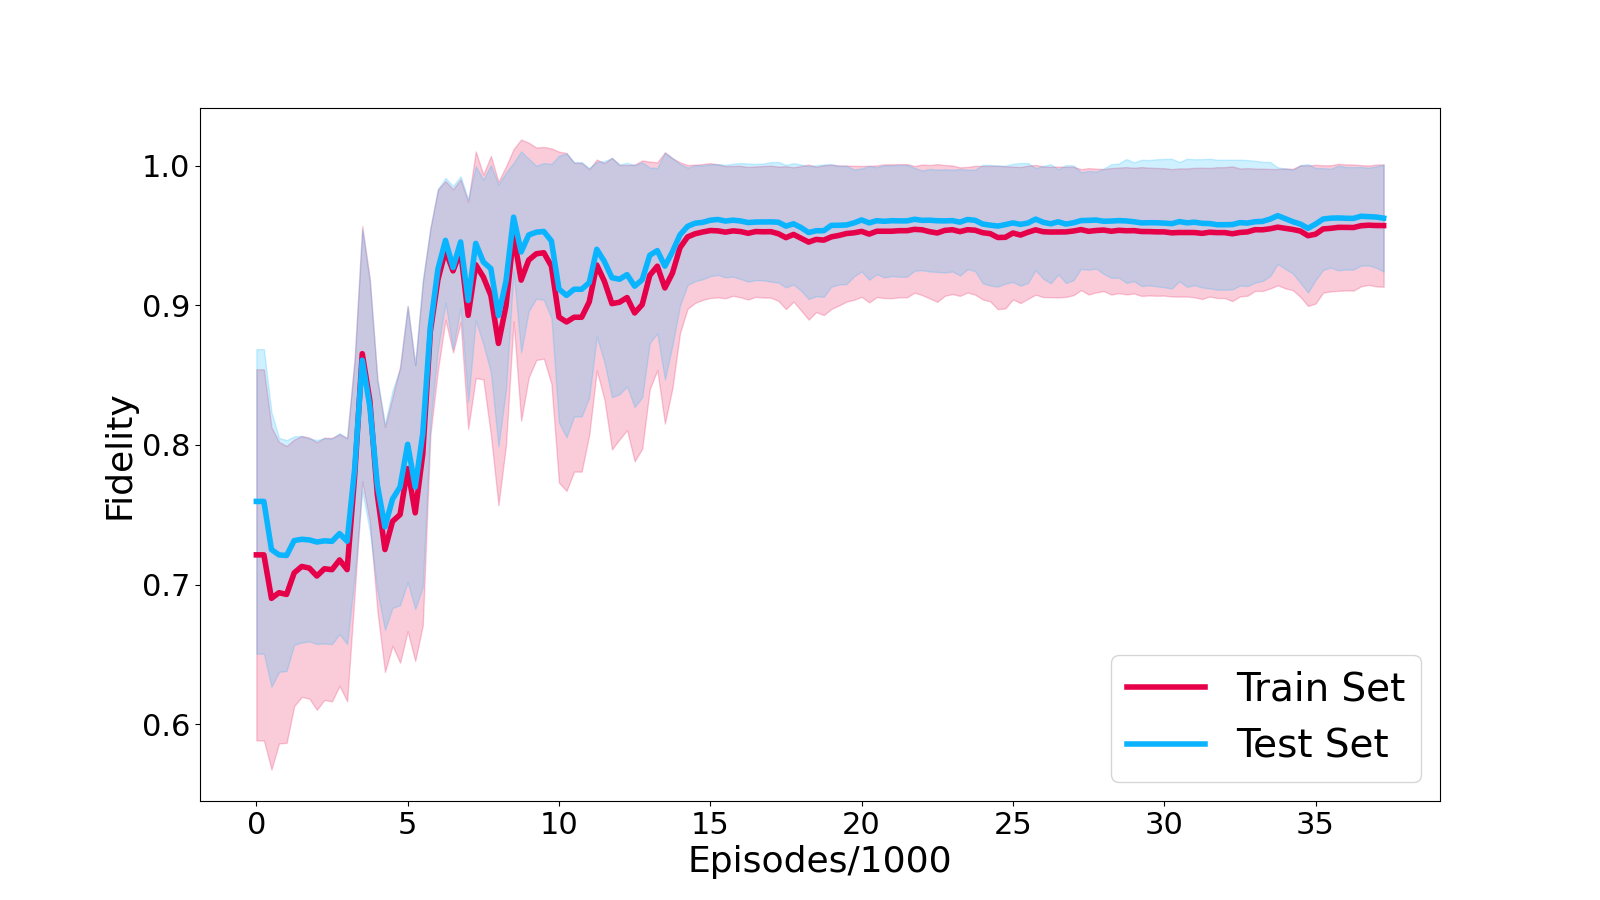
\includegraphics[width=\textwidth]{1Q_train_results.png}
    \caption{Average density matrix fidelity during training for single qubit circuits with simulated custom noise model, error bars are computed as the standard deviation.}\label{fig_1q_sim_train}
    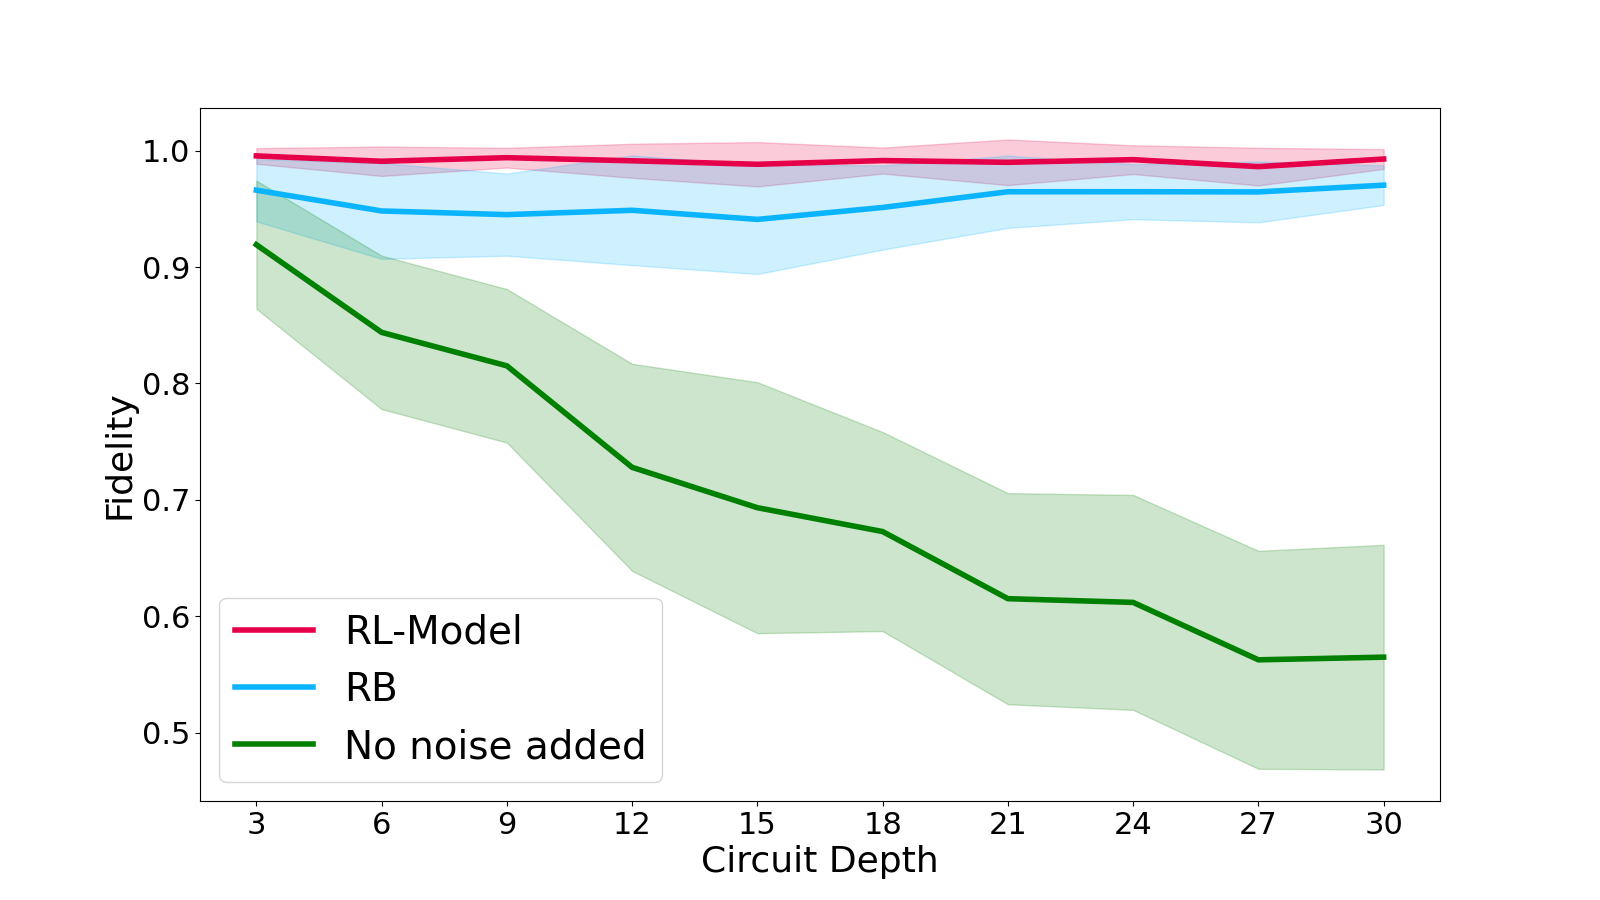
\includegraphics[width=\textwidth]{1Q_rb.png}
    \caption{Performance comparison of the RL agent with respect to the RB and the result obtained without adding any noise channel. Error bars are computed as the standard deviation.}\label{fig_1q_sim_bench}
\end{figure*}


\begin{figure*}
    \centering
    \vspace{-8mm}
    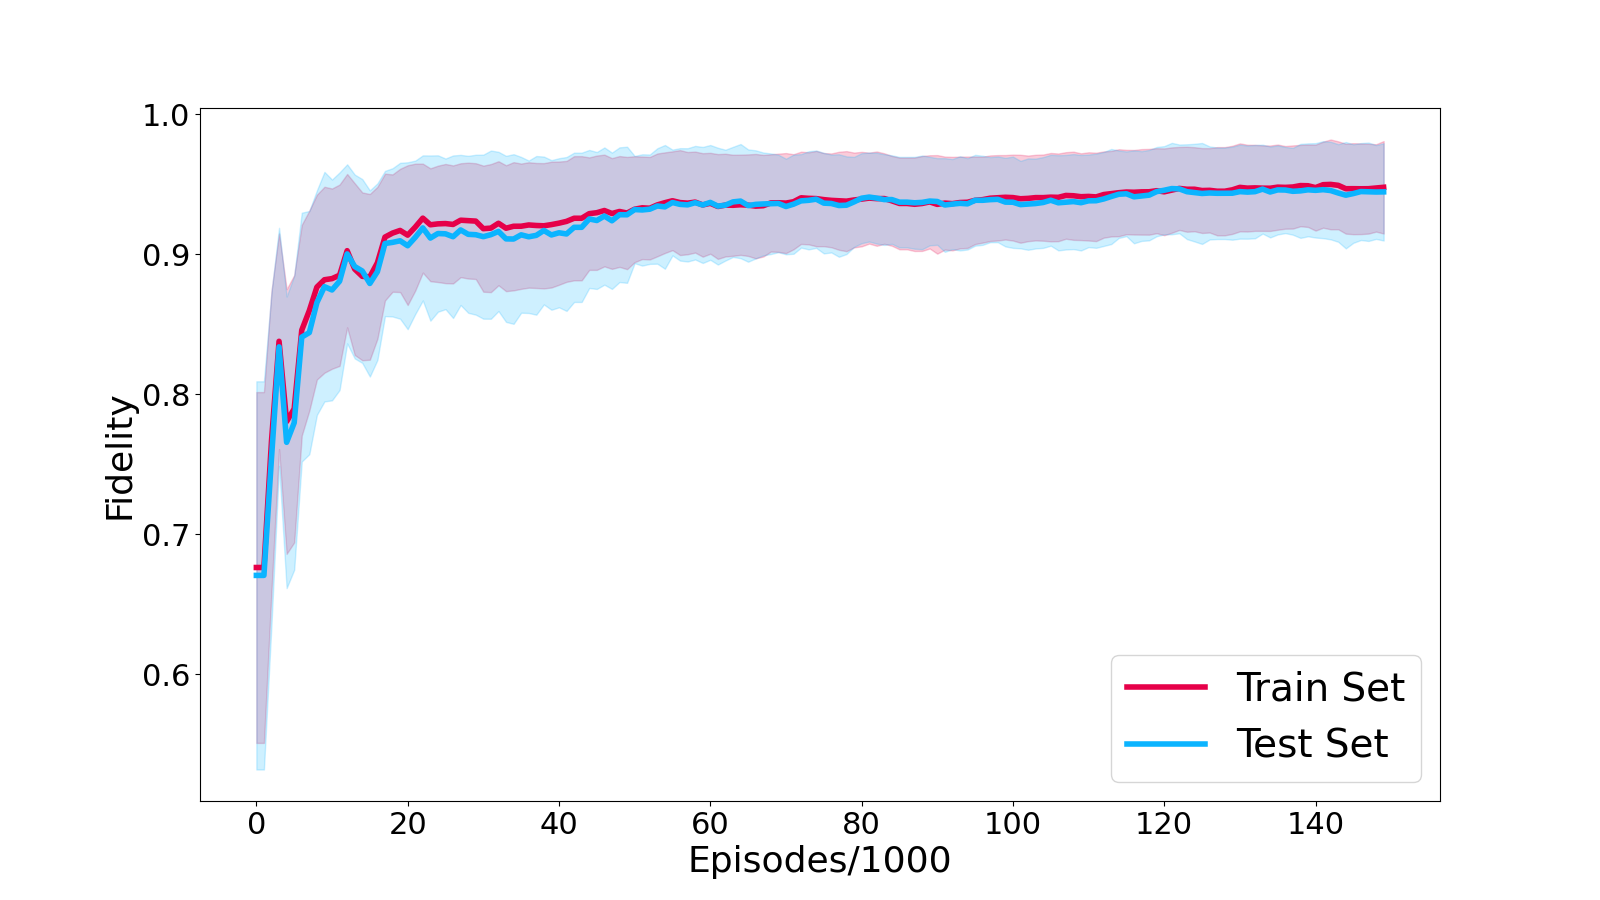
\includegraphics[width=\textwidth]{3Q_train_results.png}
    \caption{Average density matrix fidelity during training for three qubits circuits with simulated custom noise model, error bars are computed as the standard deviation.}\label{fig_3q_sim_train}
    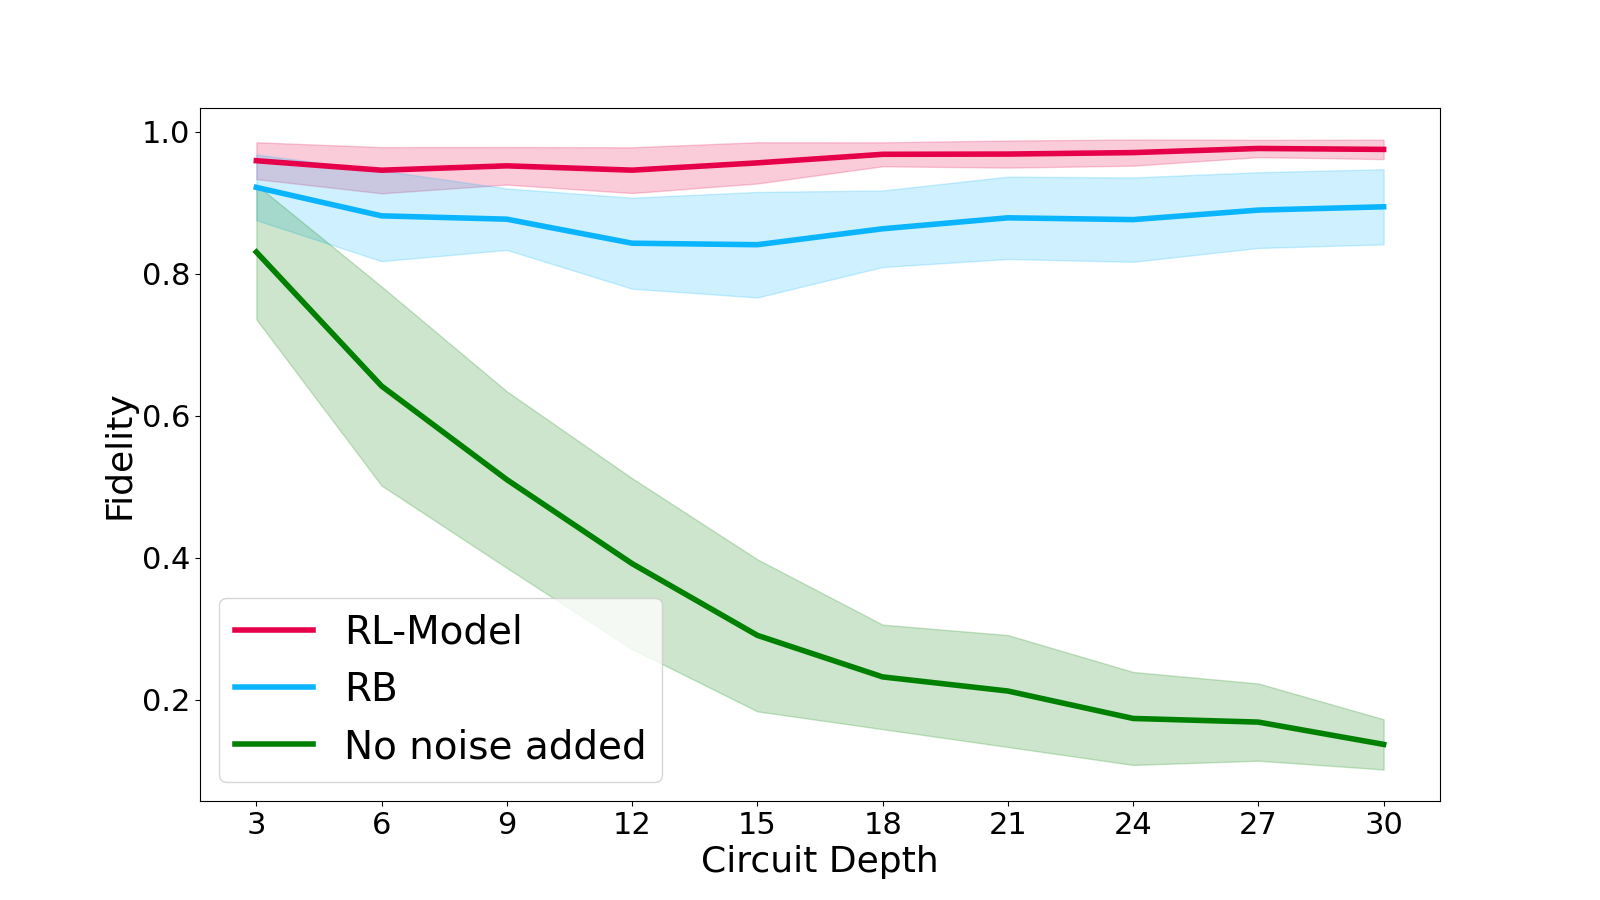
\includegraphics[width=\textwidth]{3Q_rb.png}
    \caption{Performance comparison of the RL agent with respect to the RB and the result obtained without adding any noise channel. Error bars are computed as the standard deviation.}\label{fig_3q_sim_bench}
\end{figure*}

The first simulation regards single qubit circuits with a custom noise model:
\begin{itemize}
    \item A depolarizing channel with depolarizing parameter $0.1$ is applied after each $R_z$ gate.
    \item An amplitude damping channel with decay parameter $0.05$ is applied after each $R_x$ gate.
    \item A coherent $R_x$ error is applied after each $R_x$ gate. The parameter of the coherent error rotation ($\theta^{'}$) depends on the gate rotation angle ($\theta$) as: $\theta^{'}=0.15\times\theta$.
    \item A coherent $R_z$ error is applied after each $R_z$ gate. Also in this case, the parameter of the coherent error ($\theta^{'}$) depends on the $R_z$ rotation angle ($\theta$) as: $\theta^{'}=0.1\times\theta$
\end{itemize}
This noise model is not meant to be realistic, its purpose is only to test the proposed algorithm on a noise model that depends on the gates and the rotation parameters. In order to train the RL agent, 500 random circuits of depth 7 have been generated: 400 circuits for the training set and 100 for the test set. Figure~\ref{fig_1q_sim_train} reports the average fidelity between DM as a function of the episodes, evaluated on both the training and test set.
The standard deviation over our train and test sets is represented by error bars. The agent is able to learn the simulated noise, no overfit is observed. Convergence is reached after about $1.5\cdot10^5$ episodes, when the standard deviation of the fidelity begins to shrink.\\

\noindent
In order to test the generalization properties of the model, we have tested it on random circuits of different length. Figure~\ref{fig_1q_sim_bench} reports the performance of the trained RL agent on circuits of depth spanning from 3 to 30. The RL agent has been compared with the RB and the limit case where no noise channels are added to the circuits. In order to use the RB as a noise predictor we have first extracted the decay parameter with the standard RB procedure. Then we have added a depolarizing channel with a depolarizing error equal to the decay parameter after each gate.\\
The RL agent is capable of generalizing to both longer and shorter circuits and always provides more accurate results compared to RB. This means that, as RB considers all the noise sources as depolarizing, our algorithm is able to identify the specific features of the noise. The improvement is particularly noticeable on shorter circuits, as with larger depth the noise can be approximated to a global depolarizing channel.\\

\noindent
A similar simulation has been performed to test the proposed algorithm on circuits with multiple qubits. In the noise model we have slightly reduced the parameters of the coherent errors, moreover, we have added a depolarizing channel with depolarizing error $0.02$ and an amplitude damping channel with parameter $0.08$ after each $CZ$ gate. A training set composed of 500 random three qubits circuits of depth 7 has been generated. 400 circuits for training and 100 circuits for testing. Figure~\ref{fig_3q_sim_train} reports the average density matrix fidelity during training with the standard deviation represented by error bars.
Also in this case the algorithm is able to learn the noise but convergence is much slower with respect to single qubit circuits, this is due to a bigger action space that requires more episodes to be explored. In this case convergence is reached after about $5\cdot10^6$ episodes, no overfit has been observed during the training process.\\
We have compared the performance of the RL agent with RB and with the results obtained without adding noise for circuits of different length as previously described for single qubit circuits (Fig.~\ref{fig_3q_sim_bench}). Also in this case the RL agent is capable of generalizing to circuits of different length and always provides more accurate results compared to RB. 

\subsection{Quantum hardware}\label{sec_hardware}
\begin{figure*}
    \centering
    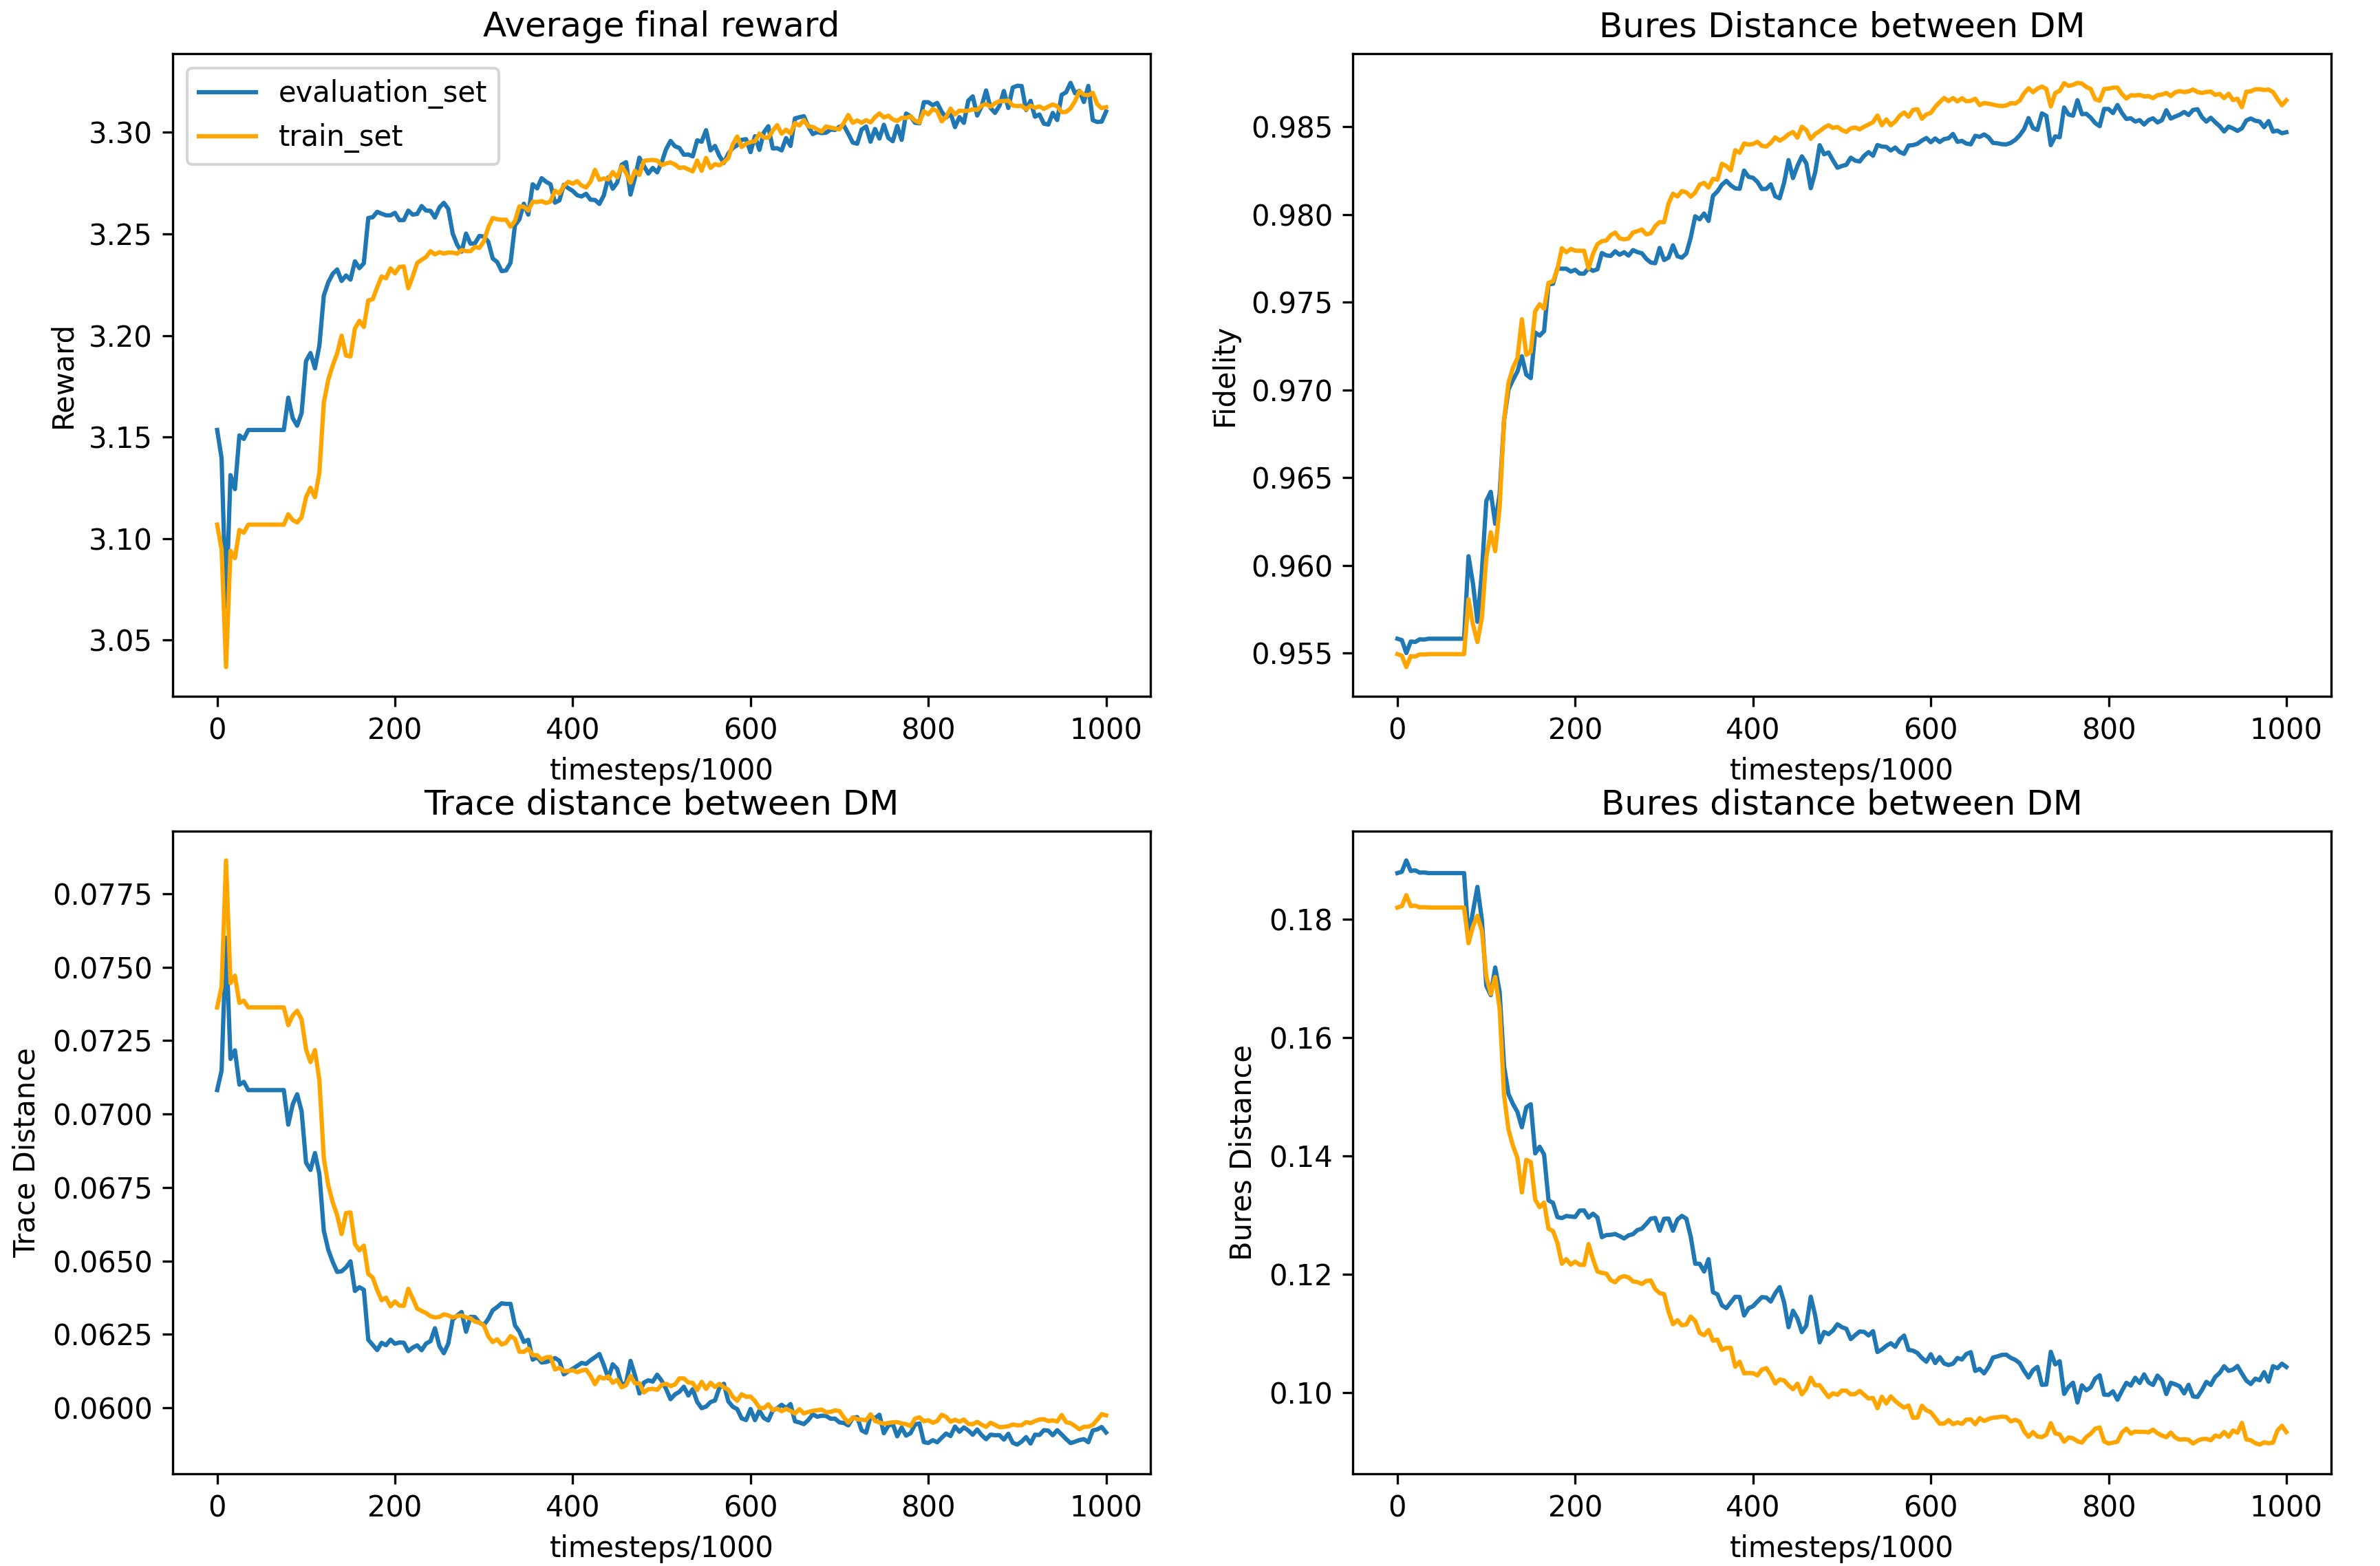
\includegraphics[width=0.6\textwidth]{training_hardware_1q.png}
    \caption{\todo{
    - REDUCE METRICS\\
    - EPISODES ON X-AXIS\\
    - CORRECT NAME OF PLOTS\\
    - ADD ERRORS AS VIOLIN PLOT OR CONFIDENCE INTERVAL}\\
    Average final reward and other evaluation metrics during training for one qubit circuits executed on quantum hardware.}\label{fig_1q_hard_train}
    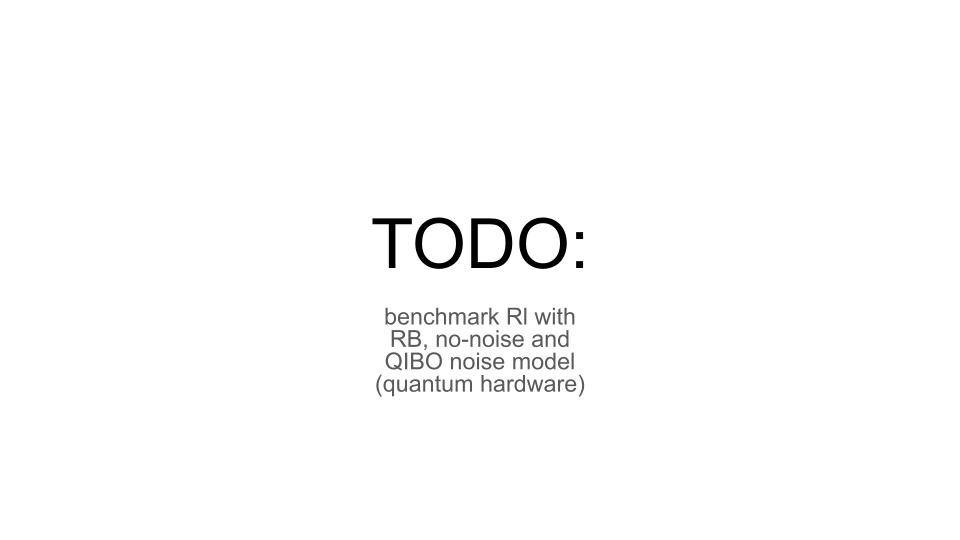
\includegraphics[width=0.6\textwidth]{benchmark_hardware_1q.png}
    \caption{\todo{ADD ALSO BENCHMARK WITH QIBO BUILT IN NOISE MODEL}
    Performance comparison of the RL agent (yellow) with respect to the RB (blue) and the result obtained without adding any noise channel (green). The performance have been computed using different metrics and for circuits of different depth.}\label{fig_1q_hard_bench}
\end{figure*}

The proposed algorithm has been tested on the quantum hardware of Technology Innovation Institute of Abu Dhabi, using a single qubit superconducting transmon chip~\cite{doi:10.1126/science.1231930}. The generated dataset is composed of 500 random circuits of depth 5, of which $20\%$ has been used as test set. In order to compute the DMs of the circuits we have used the state tomography. Moreover, to obtain more accurate DMs we have applied the readout error mitigation technique \todo{CITE}. It is important to notice that, the fidelity between the DMs of perfect circuits and the ones executed on hardware is on average $0.95$. This suggests that very little noise has accumulated during the circuit's execution, this is a different condition with respect to the simulations where a lot of noise was added to the circuits. Figure~\ref{fig_1q_hard_train} reports average final reward and other evaluation metrics during training.
The performance benchmarking of the RL agent has been performed in the same way as described in Section~\ref{sec_simulation}. Figure~\ref{fig_1q_hard_bench} reports the performance of the trained agent compared with RB, QIBO built in noise model and the circuits without noise. 

\newpage
\section{Applications} \label{sec_applications}
In this section we report two example applications of the proposed algorithm. The first application has been performed on simulations and studies the results obtained with a Quantum Fourier Transform (QFT) circuit and Grover's algorithm circuit. The second example regards an application to quantum machine learning and has been performed on TII quantum hardware. These tests are helpful to study the generalization properties of the proposed model and offer a solid stress test and benchmarking of the overall performance.

\subsection{Quantum algorithms}
The proposed model has been tested for two famous quantum algorithms, the QFT \cite{Shor_1997} and Grover's search algorithm \cite{grover1996fast}. In this test we have employed simple cases of the aforementioned algorithms in order to deal with relatively small quantum circuits. For the QFT algorithm no SWAP gates at the end of the circuit have been inserted to reverse the order of the qubits. Grover's algorithm uses one ancillary qubit and the target state is $\ket{11}$, in this way only one call of the oracle is necessary to find the target state. In both cases circuits are composed of three qubits and we have used the same noise model described in Section~\ref{sec_simulation}. The circuits have been transpiled in order to use TII native gates ($R_z$, $R_x$ and $CZ$). After the gates decomposition process, the number of gates and other important circuit parameters are reported in Table~\ref{tab_gates}.
These circuits have similar characteristics regarding the number of gates and circuit moments as the ones employed in Section~\ref{sec_simulation} for the comparison with RB. However the fraction of $CZ$ gates is different. In fact, all the circuits used for training and testing has been generated randomly using the same probability for each gate type thus contain about $1/3$ of $CZ$ gates. Moreover not all the gates contained in the transpiled circuits are Clifford as the parameters of $R_z$ and $R_x$ gates are not fixed as multiples of $\pi/2$.

\begin{table}[ht]
\centering
\caption{Number of gates and circuit moments of the transpiled circuits for QFT and Grovers's seach algorithm.}
\label{tab_gates}
\begin{tabular}{@{}llll@{}}
\toprule
& Total gates & $CZ$ gates & Moments \\
\midrule
QFT & 53 & 6 & 37 \\
Grover & 40 & 7 & 25 \\
\bottomrule
\end{tabular}
\end{table}

\noindent
For both QFT and Grover's circuits we have compared the noise model of the RL agent trained in Section~\ref{sec_simulation} with the RB noise model with the depolarizing parameter obtained in Section~\ref{sec_simulation}. 
Table~\ref{tab_results} reports the fidelity between the reconstructed density matrix and the original noisy density matrix for both the noise models. It is possible to observe that the RL agent gives better performance with respect to RB especially for the QFT circuit. \\

\begin{table}[ht]
\centering
\caption{Fidelity between the density matrix reconstructed with a noise model (RL agent or RB) and the original noisy one. The result is reported for both QFT and Grover's algorithm circuits.}
\label{tab_results}
\begin{tabular}{@{}lll@{}}
\toprule
& RL & RB \\
\midrule
QFT & 0.88 & 0.80 \\
Grover & 0.95 & 0.94 \\
\bottomrule
\end{tabular}
\end{table}

\begin{figure*}
    \centering
    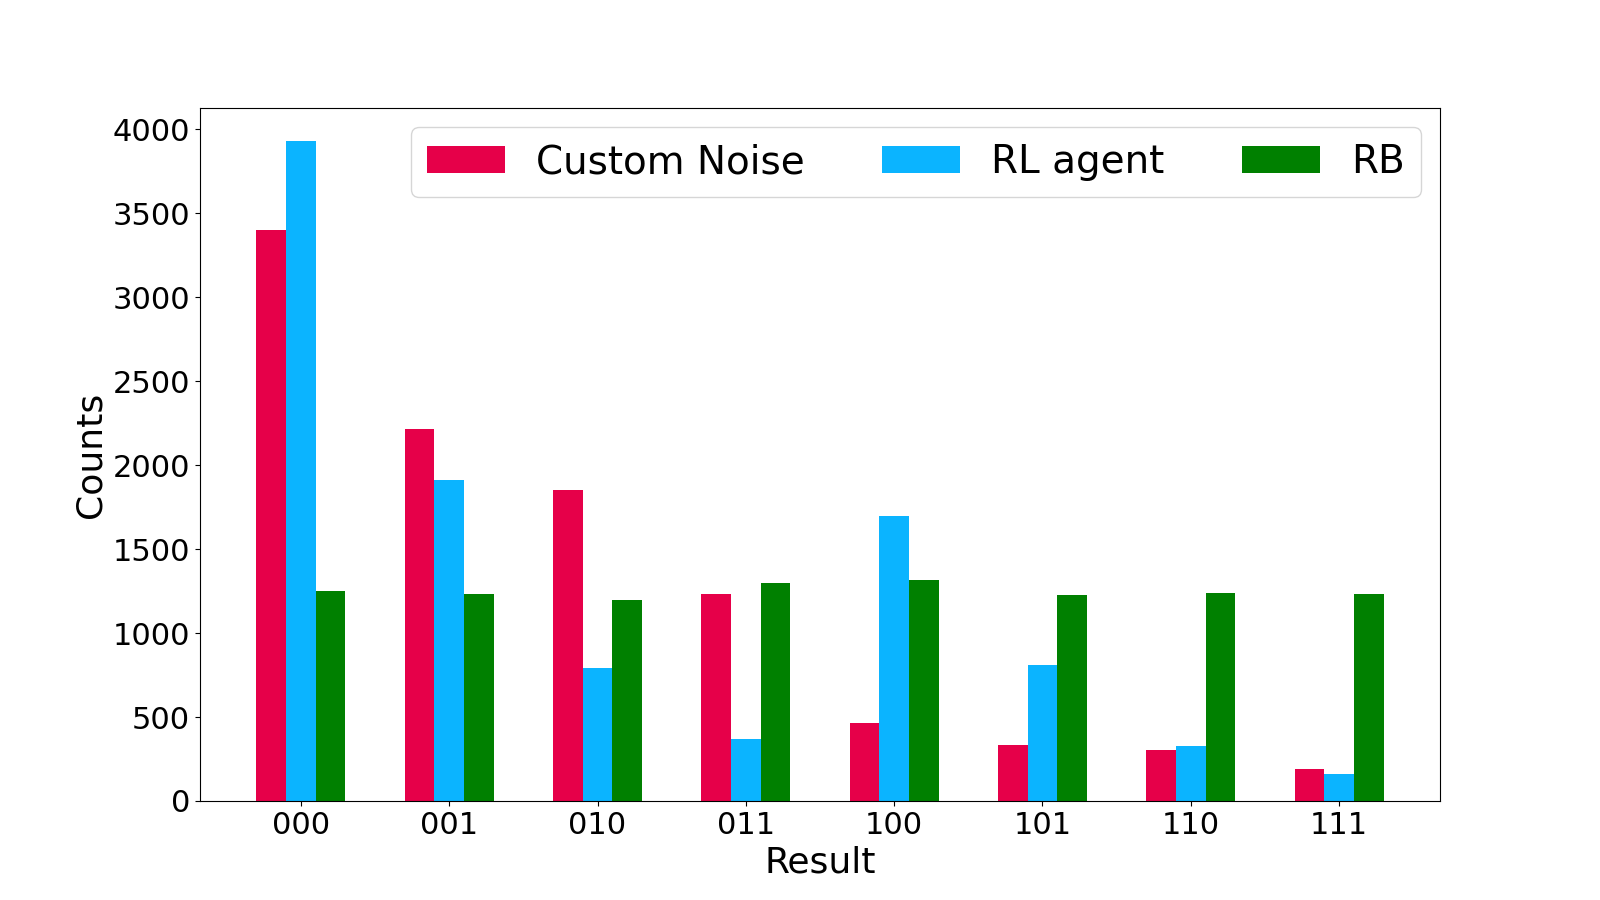
\includegraphics[width=\textwidth]{QFT_shots.png}
    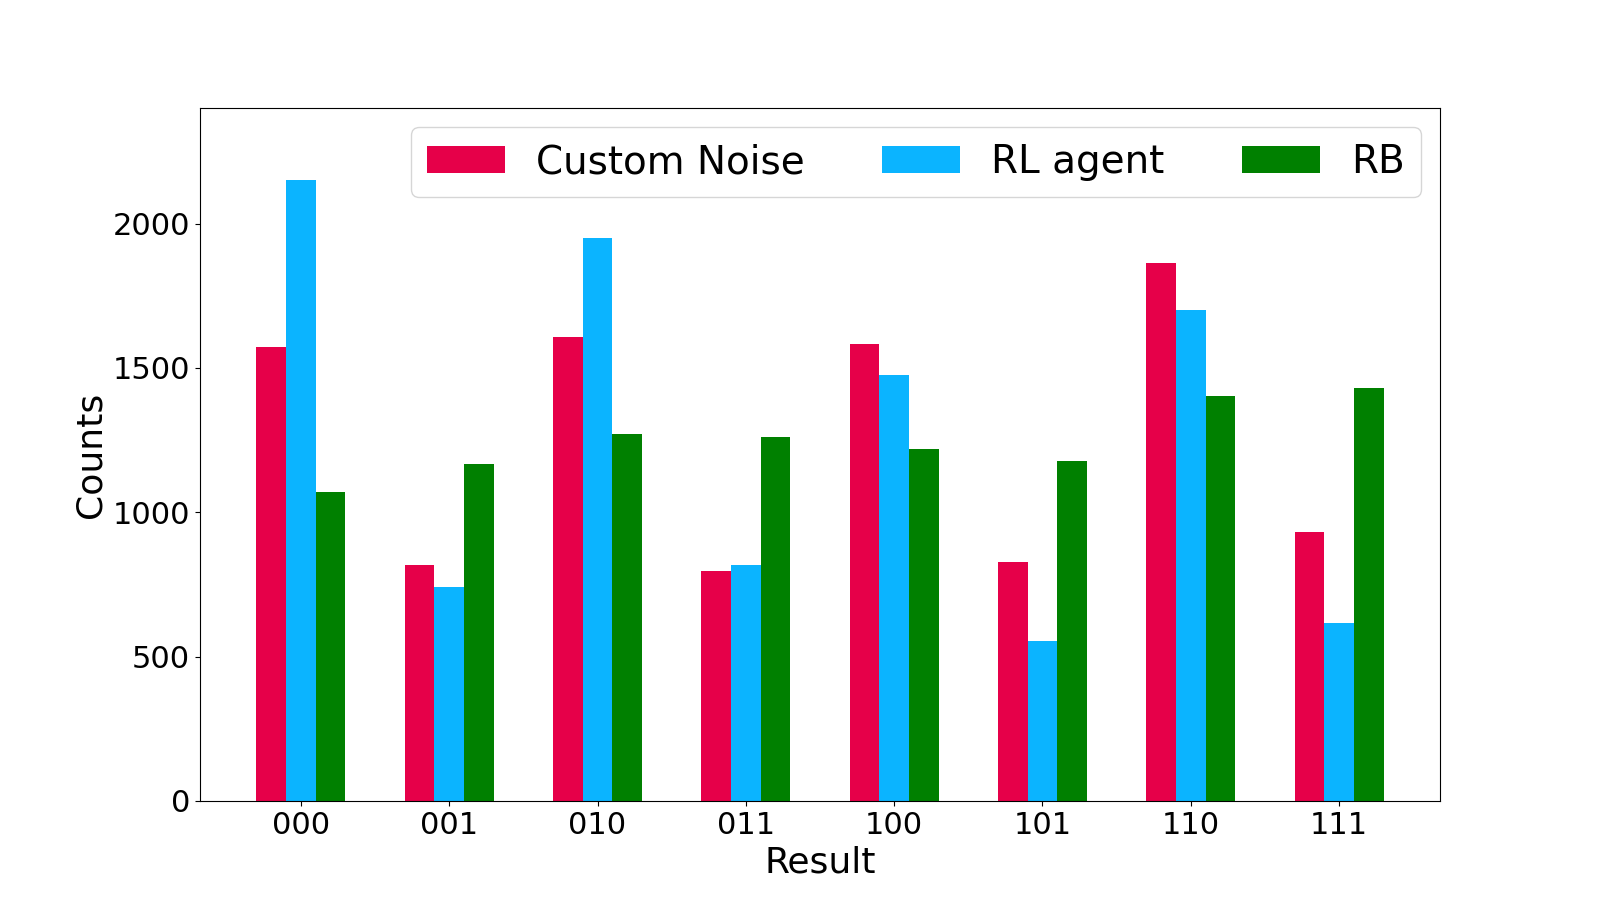
\includegraphics[width=\textwidth]{Grover_shots.png}
    \caption{Shots simulation for the three qubits QFT (top) and Grover's algorithm (bottom) quantum circuits. The histograms show a comparison between the counts obtained with the original custom noise model, the RL agent noise model and the RB noise model. For each noise model and circuit the simulation has been performed using $10^5$ shots.}\label{fig_algorithms}
\end{figure*}

\noindent
Figure \ref{fig_algorithms} shows a circuit shots simulation performed with $10^5$ shots on both QFT and Grover's algorithm circuits. In the histograms we report a comparison of the counts obtained with the original noisy circuit and the reconstructed one using the RL agent and the RB noise model. As the employed circuit are long, the RB noise model tends just to average the output. On the other hand, with the RL agent, it is possible to obtain a result that, apart for a few exceptions, is in good accordance with the shots obtained with the original noise model. In particular, this is clearly observable in the counts of the QFT simulation for the states $\ket{000}$ and $\ket{001}$. These two states are the most measured only because of the noise model (for the presence of amplitude damping channels) and this feature has been clearly reproduced by the RL agent.\\
All the results obtained in this section show that the proposed RL approach for noise modeling has good generalization properties. It can adapt to circuits with a structure different from the random ones used in the training set and with a very different length. Moreover, it is important to highlight the fact that the algorithm did not have adaptation issues when tested on circuits containing some non Clifford rotation gates.

\subsection{Quantum machine learning}

\section{Conclusions}
\todo{ADAPT FROM THESIS AND INCLUDE NEW RESULTS}
This work has presented a reinforcement learning algorithm to replicate a specific noise model of both single and multiple qubit quantum circuits. A comparative analysis between our model and the one of the standard noise characterization method, randomized benchmarking, exhibited superior performance during the simulation and quantum hardware execution.\\
The future applications of this RL model extend to noise characterization within quantum circuits. By learning the error pattern of qubits for specific gate types, the model could optimize the transpilation process~\cite{9259930}, enhancing algorithm fidelity. Moreover, it would be interesting to use the knowledge of the noise to mitigate it.
The scaling of the model to circuits with many qubits is the current biggest limitation that we aim at overcoming. To address this challenge, we are considering potential solutions. One approach might involves training the model with probability distributions derived from measurements rather than density matrices. Another solution might be partitioning into smaller circuits. This segmentation would enable parallel state tomography across multiple segments and simultaneous training of multiple models.\\
While these ideas are conceptual, and their theoretical validity should be studied deeper, the present work demonstrated that using machine learning to learn noise patterns within small quantum circuits is a proof of concept that could drive future advancements.

\backmatter

\section*{Declarations}

Some journals require declarations to be submitted in a standardised format. Please check the Instructions for Authors of the journal to which you are submitting to see if you need to complete this section. If yes, your manuscript must contain the following sections under the heading `Declarations':

\begin{itemize}
\item Funding
\item Conflict of interest/Competing interests (check journal-specific guidelines for which heading to use)
\item Ethics approval and consent to participate: Not applicable
\item Consent for publication
\item Data availability 
\item Materials availability
\item Code availability 
\item Author contribution
\end{itemize}

\noindent
If any of the sections are not relevant to your manuscript, please include the heading and write `Not applicable' for that section. 

\bibliography{sn-bibliography}

\end{document}
